\chapter{Results and discussion}
\label{sec:results_and_discussion}

	\section{Participant demographics}
	\label{sec:participant_demographics}

In total, 32 participants took part in the user study. 16 were female, 16 were male. No participant had a major visual impairment that would have caused their selection invalid. 14 participants stated they had previous experience with VR technology while the other 18 stated they had never used such technology before. Consider figures \ref{fig:results_agegroups} and \ref{fig:results_working_situation} for more information on demographics of participants.

\begin{figure}[h]
	\centering
	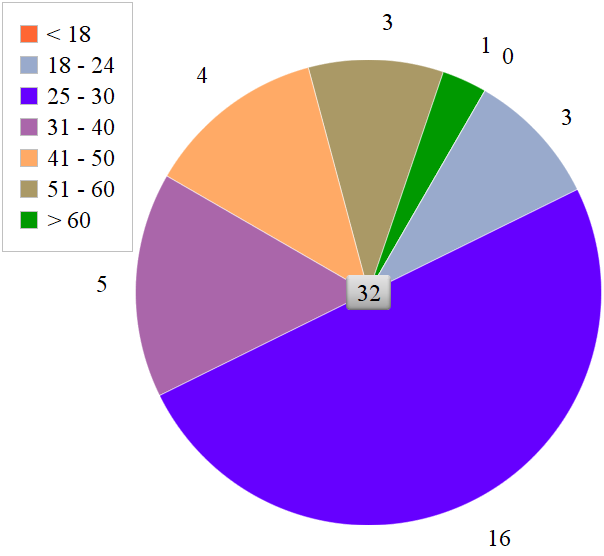
\includegraphics[width=.75\textwidth]{results_agegroups.png}\\ % PNG-File
	\caption{Age distribution of participants in the user study}
	\label{fig:results_agegroups}
\end{figure}

\begin{figure}[h]
	\centering
	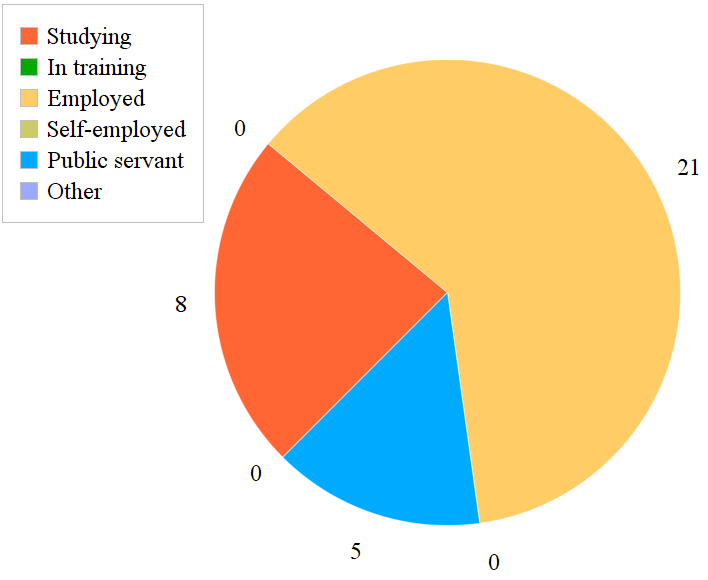
\includegraphics[width=.75\textwidth]{results_working_situation.png}\\ % PNG-File
	\caption{Working situation of participants in the user study}
	\label{fig:results_working_situation}
\end{figure}

The majority of participants was employed and between 25 and 30 years of age.

	\section{Feedback from the questionnaire}
	\label{sec:results_feedback_from_questionnaire}

As described in section \ref{sec:questionnaire}, at the end of the user study, participants were asked to rate a set of statements on a Likert-scale. Figure \ref{fig:feedback_questionnaire} shows the data gathered from this questionnaire. If a user ticked \textit{No comment} for a statement, it was not considered for these average values. The statements are shortened in this figure, the full wording can be found in \ref{sec:questionnaire} as well as an appendix.

\begin{figure}[h]
	\centering
	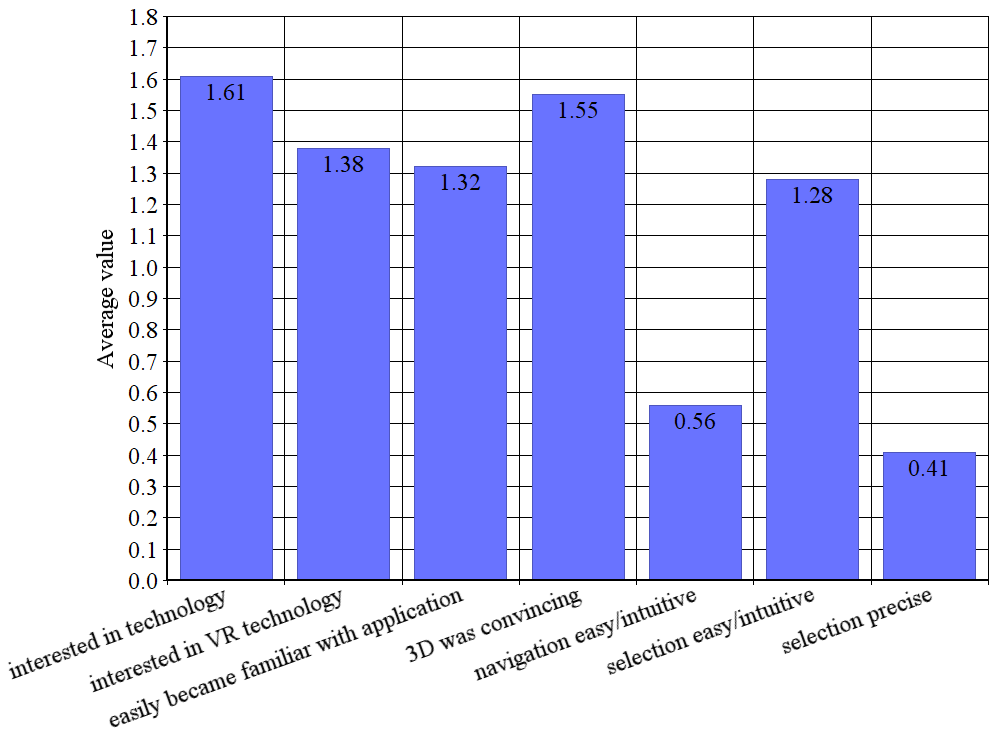
\includegraphics[width=.95\textwidth]{feedback_v2.png}\\ % PNG-File
	\caption{Feedback on the application gathered from the questionnaire. \textit{No comment} answers are not considered.}
	\label{fig:feedback_questionnaire}
\end{figure}

Figure \ref{fig:feedback_questionnaire} shows the average rating of statements on the questionnaire. Answers count as follows.

\begin{enumerate}
	\item \textit{I strongly disagree}: 2
	\item \textit{I disagree}: 1
	\item \textit{No comment}: 0
	\item \textit{I agree}: -1
	\item \textit{I strongly agree}: -2
\end{enumerate}.

Especially the precision of the selection process seemed to be not quit satisfactory to a lot of users. While the average result is still \textit{positive}, 

	\section{Individual feedback and comments}
	\label{sec:individual_feedback_and_comments}
Based on individual, informal feedback given by some participants, this section documents findings from these conversations.

\begin{itemize}
	\item The navigation shown in figure \ref{fig:feedback_questionnaire}, the navigation within the projection installation of the V2C was perceived as intuitive, easy or natural. A complete, formal description of how the navigation is designed, is not included in this work but one its general principles is that movement within the scene is always the opposite of the direction in which the user pushes the joystick of the hand-held input device, the so-called \textit{wand}. A few users have independently stated that they found this contra-intuitive and confusing.
	\item Furthermore, regarding navigation within the virtual scene, users stated that rotating the scene is confusing. The scene rotates around the user. So when a loaded object is far away from the user, rotation will cause the object to seemingly travel quickly along a horizontal circle around the user. There are ways to prevent this and rotate the object around its local z-axis but this needs practise.
	\item Regarding how the \textit{selection application} itself works, one user stated that a visible selection target with arbitrarily scalable radius would help immensely with improving the perceived precision of the selection process. As seen in figure \ref{fig:real_selection}, the selection radius around the tracked position of the hand-held input device is not visible to the user. This was a design decision with the goal of keeping the interaction individual by not rendering semi-transparent, unnatural objects, however it is understandable that users who desire maximum precision would want have the selection radius visible and adjustable at all times.
\end{itemize}

	\section{Saliency and difference maps}
	\label{sec:saliency_and_difference_maps}
This section contains figures depicting \textit{mesh saliency} and \textit{user saliency} maps for each object as well as \textit{unweighted} (raw) and \textit{weighted} difference maps. For each object, these maps are shown in three angles, front, side and top. All figures are orthographic renderings. The scale shown in figure \ref{fig:results_scale} is used for all figures. Note that it is uniform in the sense that the color mapping represents values between 0.0 and 1.0. For saliency maps, this expresses the saliency (the \textit{perceived importance} per vertex), for difference maps it expresses the differenc between saliency maps vertex wise.

\begin{figure}[htb]
	\centering
	
\includegraphics[width=.7\textwidth]{result_maps/scale_values.png}\\ % PNG-File
	\caption{The uniform scale used for figures in this section.}
	\label{fig:results_scale}
\end{figure}

\FloatBarrier
		\subsection{Bunny}
		\label{sec:results_bunny}
%
%	BUNNY
%
\begin{figure}[!htb]
	\centering
	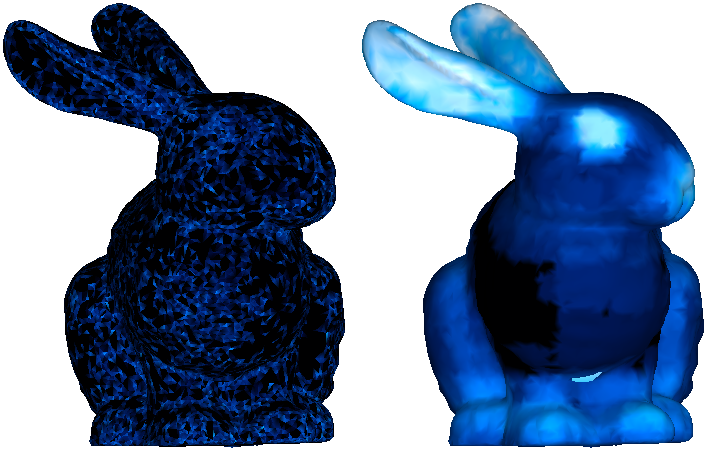
\includegraphics[width=.7\textwidth]{result_maps/bunny/bunny_front_A.png}\\ % PNG-File
	\caption{Normalised saliency maps for the first model, orthographic front view. Left: \textit{mesh saliency}, right: \textit{user saliency}}
	\label{fig:results_bunny_front_a}
\end{figure}
\begin{figure}[!htb]
	\centering
	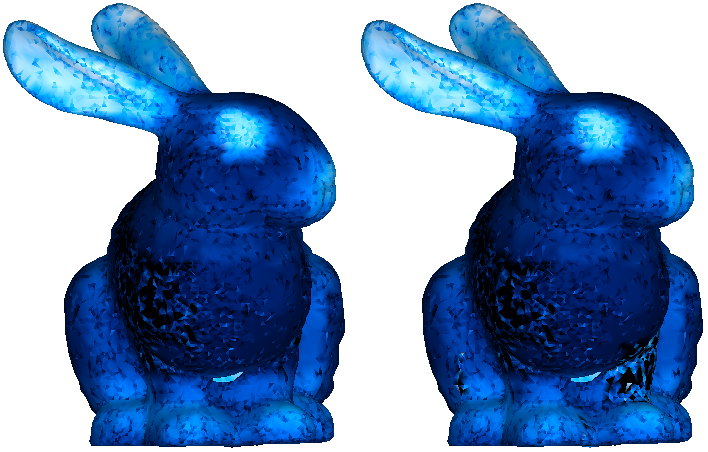
\includegraphics[width=.7\textwidth]{result_maps/bunny/bunny_front_B.png}\\ % PNG-File
	\caption{Normalised difference maps for the first model, orthographic front view. Left: \textit{unweighted differences}, right: \textit{weighted differences}}
	\label{fig:results_bunny_front_b}
\end{figure}

\begin{figure}[!htb]
	\centering
	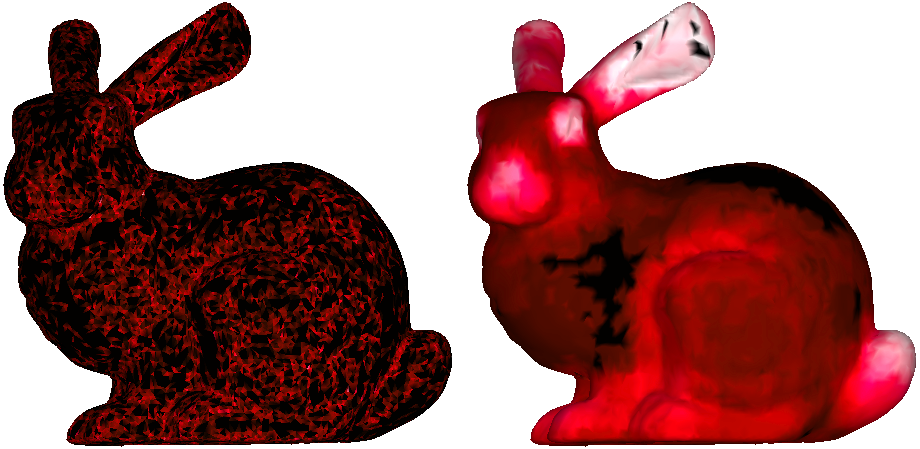
\includegraphics[width=.85\textwidth]{result_maps/bunny/bunny_side_A.png}\\ % PNG-File
	\caption{Normalised saliency maps for the first model, orthographic side view. Left: \textit{mesh saliency}, right: \textit{user saliency}}
	\label{fig:results_bunny_side_a}
\end{figure}
\begin{figure}[!htb]
	\centering
	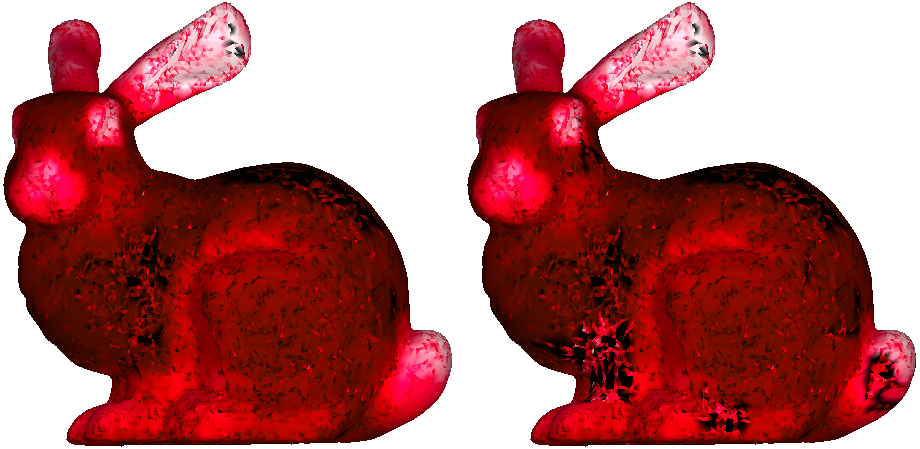
\includegraphics[width=.85\textwidth]{result_maps/bunny/bunny_side_B.png}\\ % PNG-File
	\caption{Normalised difference maps for the first model, orthographic side view. Left: \textit{unweighted differences}, right: \textit{weighted differences}}
	\label{fig:results_bunny_side_b}
\end{figure}

\begin{figure}[!htb]
	\centering
	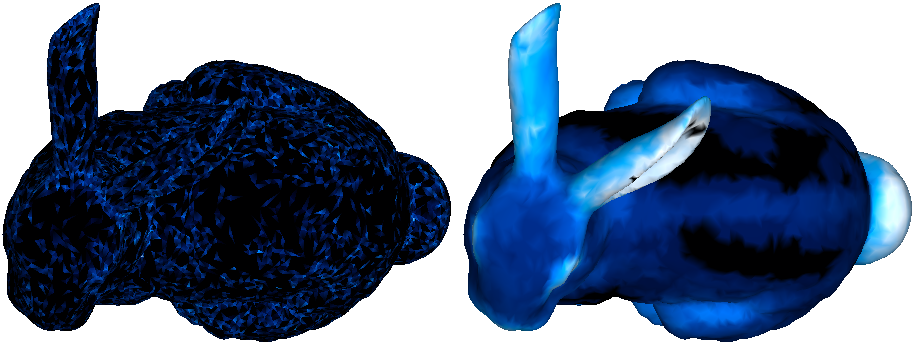
\includegraphics[width=.9\textwidth]{result_maps/bunny/bunny_top_A.png}\\ % PNG-File
	\caption{Normalised saliency maps for the first model, orthographic top view. Left: \textit{mesh saliency}, right: \textit{user saliency}}
	\label{fig:results_bunny_top_a}
\end{figure}
\begin{figure}[!htb]
	\centering
	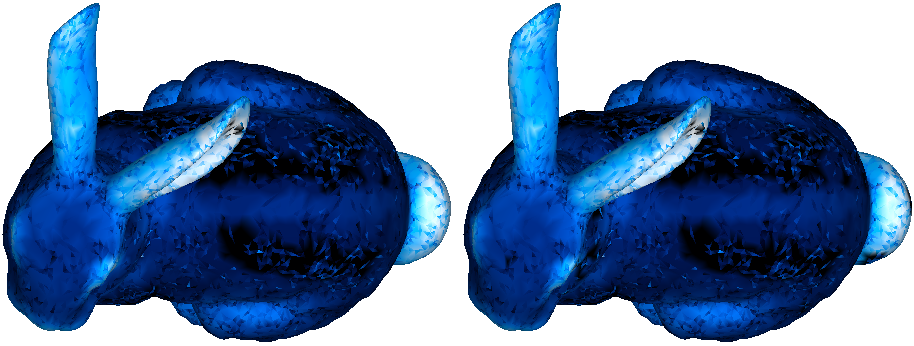
\includegraphics[width=.9\textwidth]{result_maps/bunny/bunny_top_B.png}\\ % PNG-File
	\caption{Normalised difference maps for the first model, orthographic top view. Left: \textit{unweighted differences}, right: \textit{weighted differences}}
	\label{fig:results_bunny_top_b}
\end{figure}

\FloatBarrier
		\subsection{Cow}
		\label{sec:results_cow}
%
%	COW
%
\begin{figure}[!htb]
	\centering
	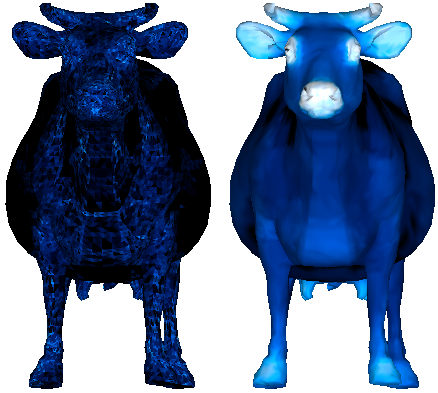
\includegraphics[width=.55\textwidth]{result_maps/cow/cow_front_A.png}\\ % PNG-File
	\caption{Normalised saliency maps for the second model, orthographic front view. Left: \textit{mesh saliency}, right: \textit{user saliency}}
	\label{fig:results_cow_front_a}
\end{figure}
\begin{figure}[!htb]
	\centering
	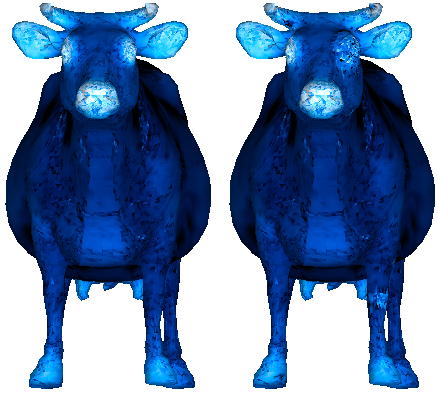
\includegraphics[width=.55\textwidth]{result_maps/cow/cow_front_B.png}\\ % PNG-File
	\caption{Normalised difference maps for the second model, orthographic front view. Left: \textit{unweighted differences}, right: \textit{weighted differences}}
	\label{fig:results_cow_front_b}
\end{figure}

\begin{figure}[!htb]
	\centering
	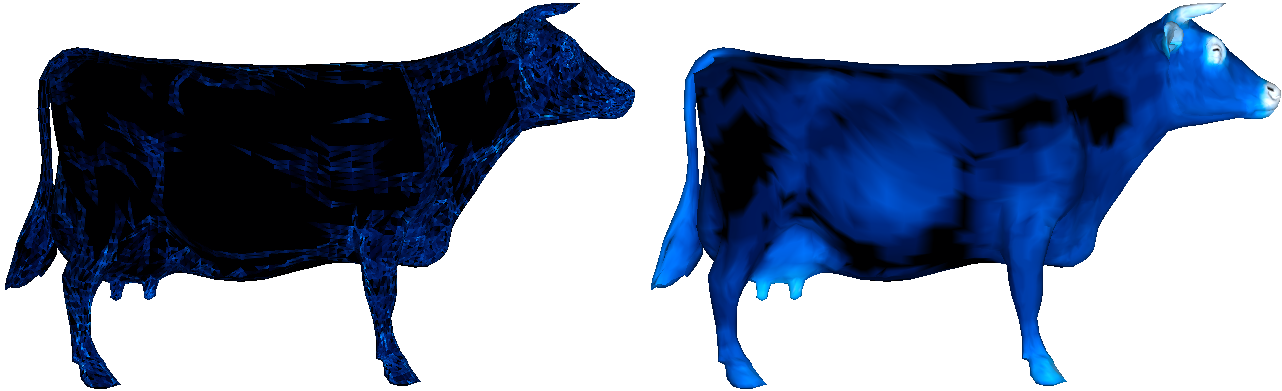
\includegraphics[width=1.0\textwidth]{result_maps/cow/cow_side_A.png}\\ % PNG-File
	\caption{Normalised saliency maps for the second model, orthographic side view. Left: \textit{mesh saliency}, right: \textit{user saliency}}
	\label{fig:results_cow_side_a}
\end{figure}
\begin{figure}[!htb]
	\centering
	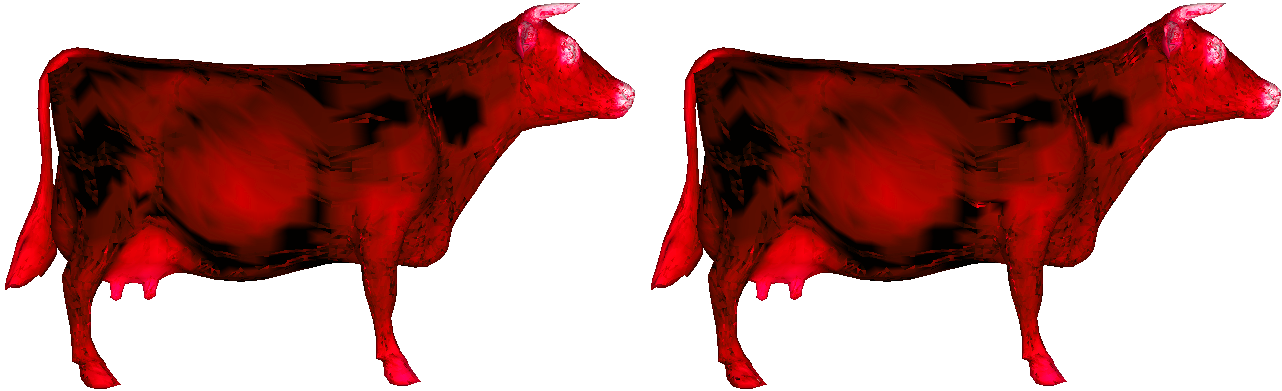
\includegraphics[width=1.0\textwidth]{result_maps/cow/cow_side_B.png}\\ % PNG-File
	\caption{Normalised difference maps for the second model, orthographic side view. Left: \textit{unweighted differences}, right: \textit{weighted differences}}
	\label{fig:results_cow_side_b}
\end{figure}

\begin{figure}[!htb]
	\centering
	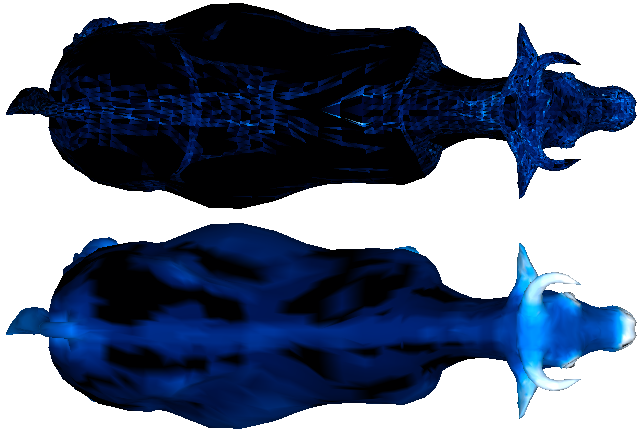
\includegraphics[width=.7\textwidth]{result_maps/cow/cow_top_A.png}\\ % PNG-File
	\caption{Normalised saliency maps for the second model, orthographic top view. Top: \textit{mesh saliency}, bottom: \textit{user saliency}}
	\label{fig:results_cow_top_a}
\end{figure}
\begin{figure}[!htb]
	\centering
	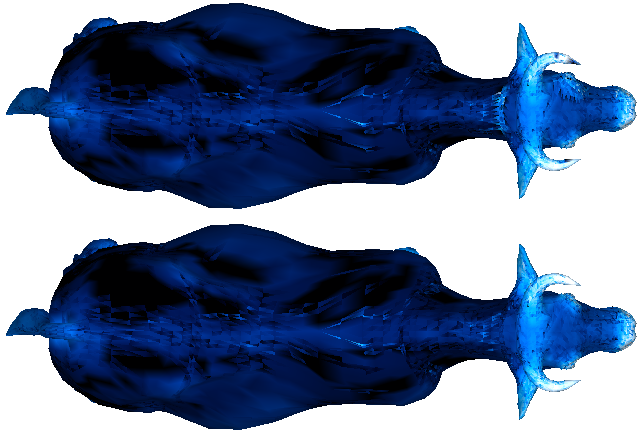
\includegraphics[width=.7\textwidth]{result_maps/cow/cow_top_B.png}\\ % PNG-File
	\caption{Normalised difference maps for the second model, orthographic top view. Top: \textit{unweighted differences}, bottom: \textit{weighted differences}}
	\label{fig:results_cow_top_b}
\end{figure}

\FloatBarrier
		\subsection{P51}
		\label{sec:results_p51}
%
%	P51
%
\begin{figure}[!htb]
	\centering
	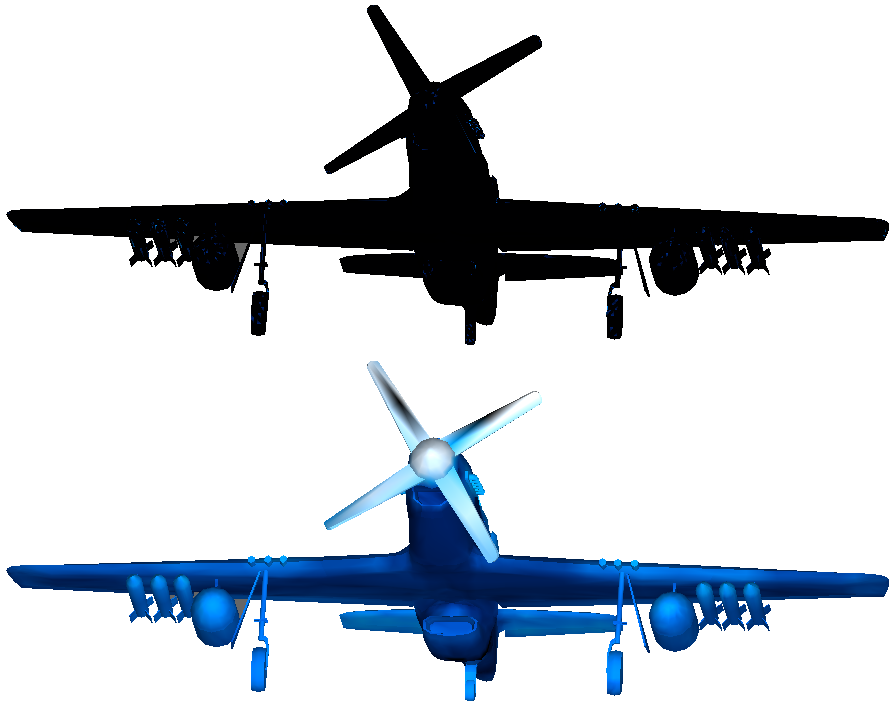
\includegraphics[width=.7\textwidth]{result_maps/P51/P51_front_A.png}\\ % PNG-File
	\caption{Normalised saliency maps for the third model, orthographic front view. Top: \textit{mesh saliency}, bottom: \textit{user saliency}}
	\label{fig:results_p51_front_a}
\end{figure}
\begin{figure}[!htb]
	\centering
	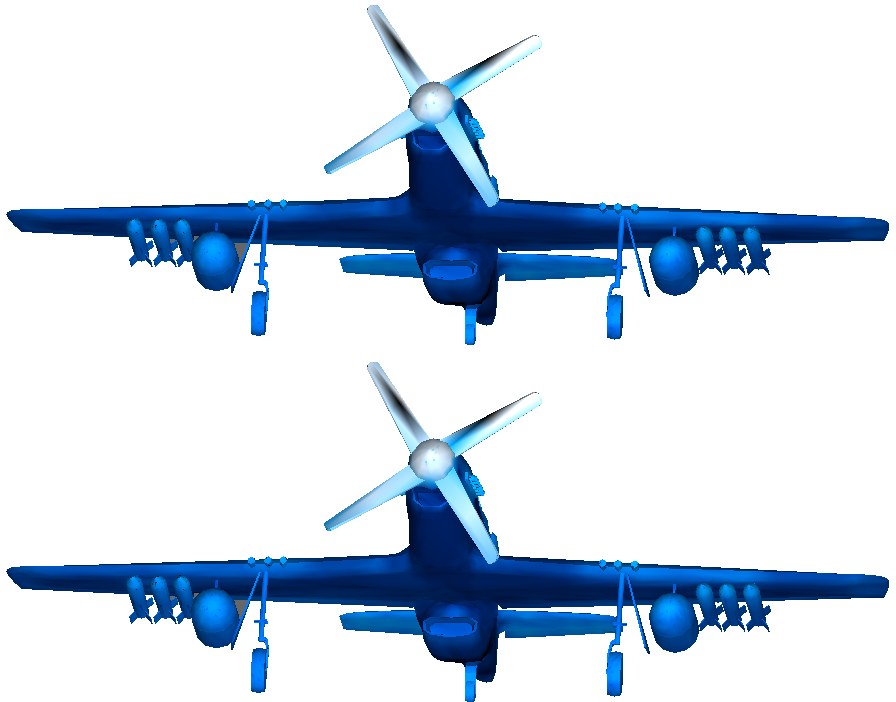
\includegraphics[width=.7\textwidth]{result_maps/P51/P51_front_B.png}\\ % PNG-File
	\caption{Normalised difference maps for the third model, orthographic front view. Top: \textit{unweighted differences}, bottom: \textit{weighted differences}}
	\label{fig:results_p51_front_b}
\end{figure}

\begin{figure}[!htb]
	\centering
	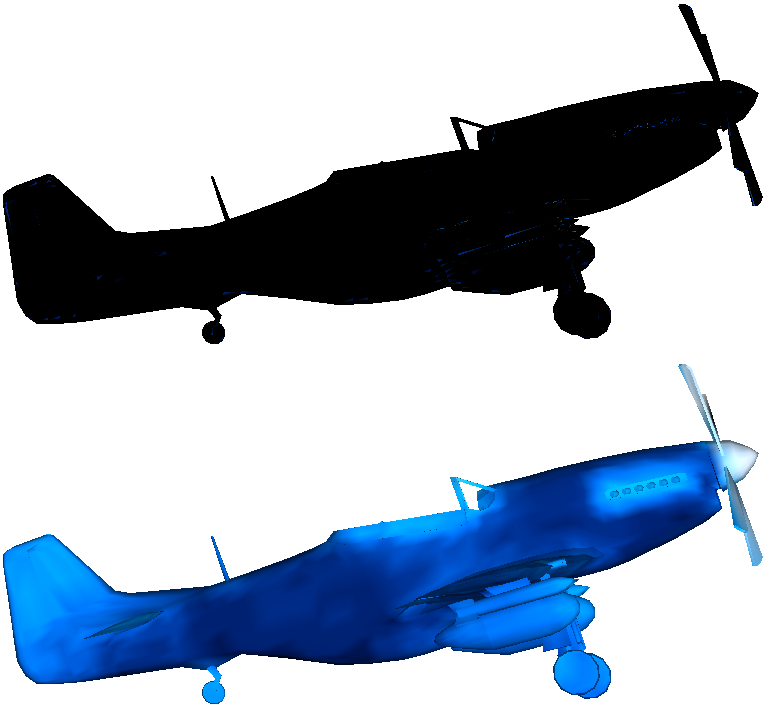
\includegraphics[width=.65\textwidth]{result_maps/P51/P51_side_A.png}\\ % PNG-File
	\caption{Normalised saliency maps for the third model, orthographic side view. Top: \textit{mesh saliency}, bottom: \textit{user saliency}}
	\label{fig:results_p51_side_a}
\end{figure}
\begin{figure}[!htb]
	\centering
	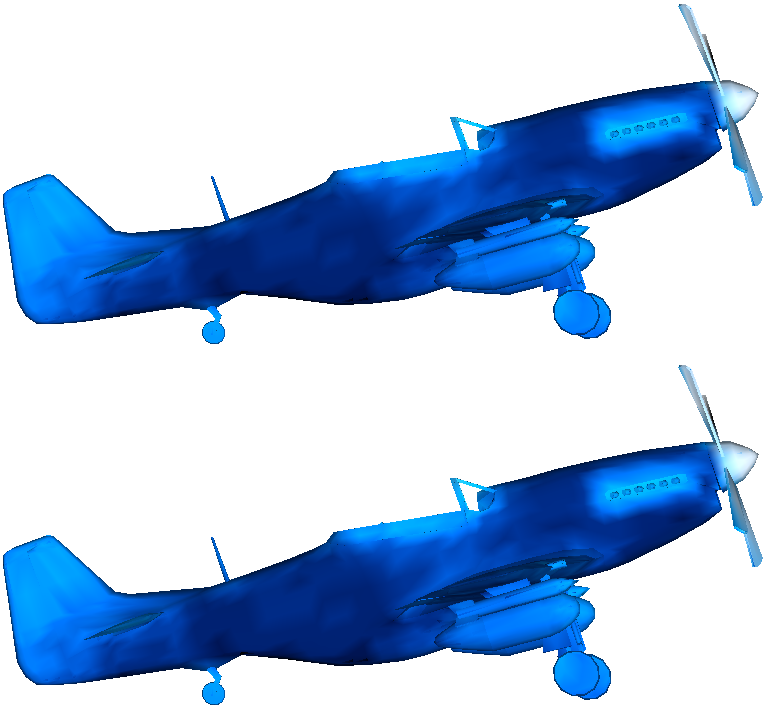
\includegraphics[width=.65\textwidth]{result_maps/P51/P51_side_B.png}\\ % PNG-File
	\caption{Normalised difference maps for the third model, orthographic side view. Top: \textit{unweighted differences}, bottom: \textit{weighted differences}}
	\label{fig:results_p51_side_b}
\end{figure}

\begin{figure}[!htb]
	\centering
	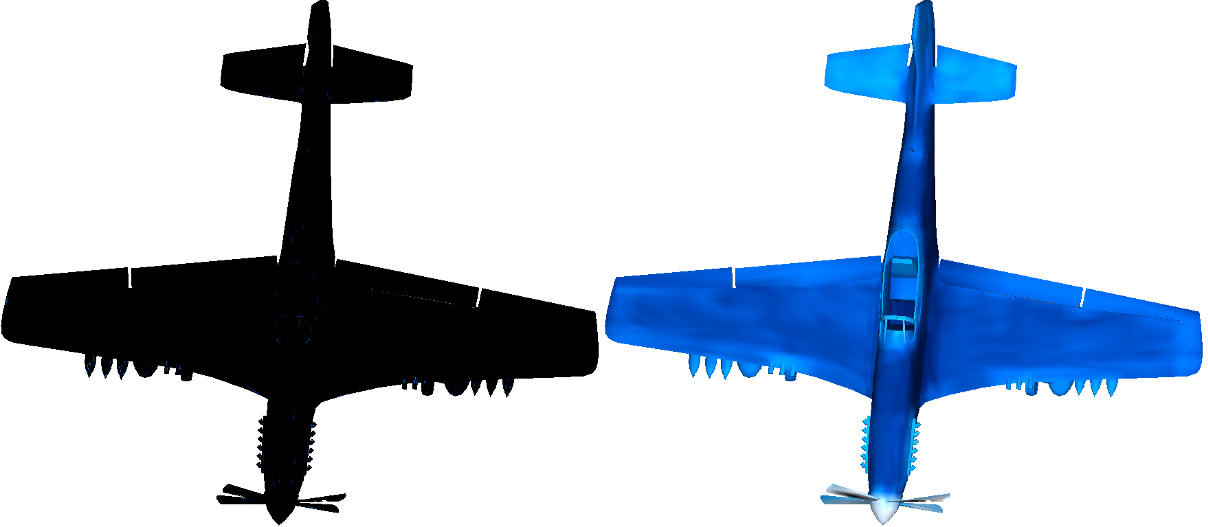
\includegraphics[width=.9\textwidth]{result_maps/P51/P51_top_A.png}\\ % PNG-File
	\caption{Normalised saliency maps for the third model, orthographic top view. Left: \textit{mesh saliency}, right: \textit{user saliency}}
	\label{fig:results_p51_top_a}
\end{figure}
\begin{figure}[!htb]
	\centering
	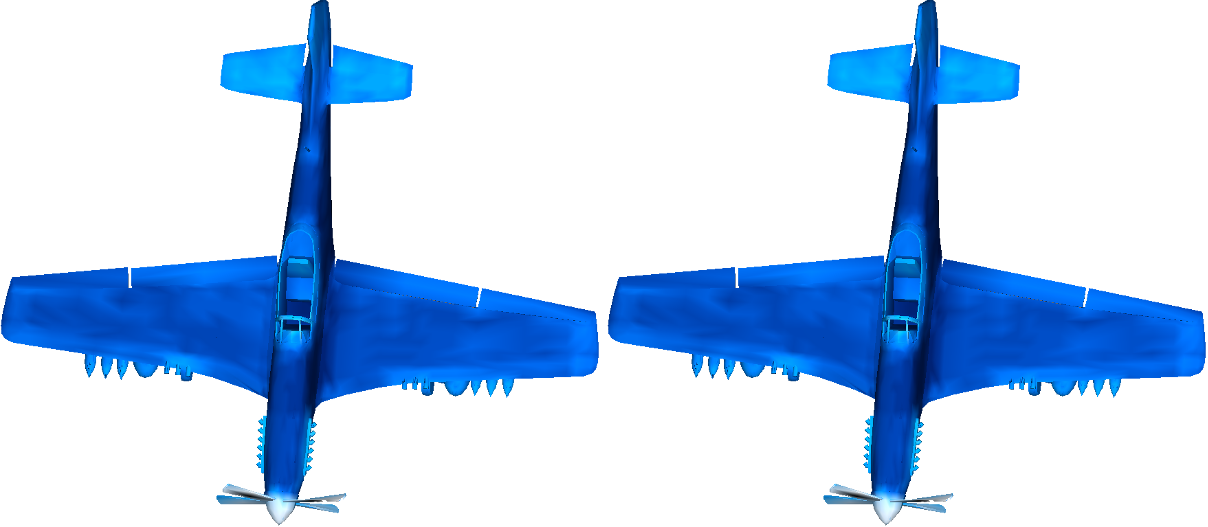
\includegraphics[width=.9\textwidth]{result_maps/P51/P51_top_B.png}\\ % PNG-File
	\caption{Normalised difference maps for the third model, orthographic top view. Left: \textit{unweighted differences}, right: \textit{weighted differences}}
	\label{fig:results_p51_top_b}
\end{figure}
%
%	ENDE BILDER
%
\FloatBarrier

	\section{Evaluation of differences}
	\label{sec:evaluation_of_differences}
This section contains quantitative observations of the resulting saliency and difference maps as well as a discussion of the measure of difference as suggested in section \ref{sec:measure_of_difference}. Based on observations described here, it is fair to say that the measure of difference is not expressive enough and is not suitable to describe differences between user selections and results achieved through \textit{mesh saliency} in a sound way.

		\subsection{Measure of difference}
		\label{sec:measure_of_difference}
Table \ref{tab:results_results_table} shows the results of using the measure of difference as well as additional information about the three 3D models used for this work. The following abbreviations are used:

\begin{align*}
Dif_{raw} &= \frac
	{
		\sum_{i \in V_{o})}
			\Delta_{raw}(v_i)
	}{
		V_{o}
	}
\end{align*}

\begin{align*}
Dif_{weighted} &= \frac
	{
		\sum_{i \in V_{o})}
			\Delta_{weighted}(v_i)
	}{
		V_{o}
	}
\end{align*}

Where, for a given object $o$, $V_{o}$ is the total number of vertices contained in $o$ and $\Delta_{raw}(v_i)$ is the absolute value of the difference between the computed \textit{mesh saliency} $S_{M}(v_i)$ value and the average \textit{user saliency value} $S_{U}(v_i)$ for vertex $v_i$.

\begin{table}[]
\begin{tabular}{l|llllll}
Model &	Vertices total &		Vertices weighted &	$Dif_{raw}$ &			$Dif_{weighted}$ &	$n*\epsilon$	\\ \hline
Bunny &	68,754 &			2,667 &			0.23435 &			0.234545 &		4			\\
Cow &	69,648 &			3,200 &			0.27431 &			0.269036 &		4			\\
P51 &	51,708 &			0 &			0.38002	&			0.38002 &		1				\\
\end{tabular}
\caption{Resulting differences and information on the 3D models}\label{tab:results_results_table}
\end{table}
% table 6.1

In other words, $Dif_{raw}$ and $Dif_{weighted}$ can be interpreted as a percent number which expresses how much the average user selection differs from the computed mesh saliency map for a given object. In the case of the first model, Bunny, both the raw, unweighted and weighted overall difference amounts to roughly 23\%. The difference only affects decimal places after the third one after the comma. For the second model, the raw overall difference amounts to about 27\%, as does the weighted overall difference when rounded. For the third model, both ratios are the exact same at about 38\%. $n$ is the factor of $\epsilon$ used for computation of \textit{mesh saliency} values for the objects where $\epsilon$ is 0.3\% of the main diagonal of the object's bounding box.

The \textit{mesh saliency} maps were computed using \texttt{climberpi's} implementation \cite{clms} of of the original procedure suggested in \cite{lee2005mesh}. It is implemented strictly following the concept yet, obviously, I was not able to achieve saliency maps that look similar to those included in the original paper. In the original paper, the authors suggest using scales $\sigma_{n} \in {1\epsilon, 2\epsilon, 3\epsilon, 4\epsilon, 5\epsilon, 6\epsilon, }$. As shown in table \ref{tab:results_results_table}, different values for the objects were used in order to get somewhat plausible \textit{mesh saliency} maps. Trying multiple variations of $n$, where $n*\epsilon = \sigma_{n}$ did not lead to results much more convincing.

A is a major shortcoming of the measure of difference is the fact that every saliency value is normalised to range $[0, 1]$. As stated before, this was done with the goal of describing how much the user selection differs from the results of \textit{mesh saliency} in percentage. However, the problem with dividing each individual saliency value by the highest value found is that a large number of near-zero saliency values is a result. This is obvious when considering figures \ref{fig:results_bunny_front_a}, \ref{fig:results_bunny_side_a} and all the other images containing computed \textit{mesh saliency} maps. The majority of values seems to be close to zero, resulting in most of what is visible shaded in black or a very dark blue. The most extreme extent to which this behavior can occur is shown in the figures depicting the third model in section \ref{sec:results_p51}. For more details on why \textit{mesh saliency} - in its originally proposed, unaltered state - does not produce quality results for mechanical objects, see section \ref{sec:mesh_saliency_with_mechanical_objects}.

		\subsection{Observation of saliency maps}
		\label{sec:mesh_saliency_with_mechanical_objects}
When considering the average \textit{user saliency} maps, four major observations are to be described. First, while \textit{mesh saliency} maps still look very different, a general common theme as to which parts are more important and which are not, is there - especially when it comes to contours, geometrical details and \textit{characteristic} parts of the objects. For models Bunny and Cow, a strong emphasis on the entire head part is noticeable, with a much stronger variation in values in the \textit{user saliency} map. Again, a resemblance in general can be noted, but it is obvious that users had much more complex criteria for their selection than solely local curvature differences computed for on a per-vertex basis. This results in prominent differences in saliency maps, hardly possible to describe solely by numbers and ratios. Distinct patches of higher perceived importance by users contradict, in part, the results of \textit{mesh saliency}. For example, the belly region of the second model (Cow) was marked as \textit{important} by about 40\% of users, whereas it is entirely \textit{uninteresting} according to \textit{mesh saliency}.

Second, within \textit{user saliency} maps, seemingly zero-saliency patches can be found in the middle of cohesive parts of objects that seem to have been selected by almost 100\% of participants. This behavior is especially prominent, for example, in the ear region of model one (Bunny) as well as the eye and snout part of model two (Cow). Model one lacks the perfect axial symmetry of models two and three, which might, in part, explain stronger variations in user selections but still, this behavior being caused by vague, \textit{lazy} user selections is not highly believable. However, observing the \textit{user saliency} map of model two, reveals that the small, seemingly zero-saliency \textit{spot} only appears on one side of the head. This is further reason to assume this behavior is not caused by users. As described in section \ref{sec:testing_setup}, I took steps trying to ensure that the \textit{selection application's} implementation works correctly as much as possible, however it has not been verified on a conceptual, mathematical level. Minor bugs and weaknesses of the implementation can not be ruled out as a cause for this behavior. Lastly, the visual feedback to what is currently selected and what is not, might be another factor contributing to this behavior. If shading all currently selected vertices was not clear or precise enough, caused by interpolation between extremely close vertices, this might be another factor causing these zero-saliency spots.

Third, \textit{user saliency} maps seem to very much more strongly regarding the range of values. Put simply, \textit{mesh saliency} maps seem to only contain patches that are not interesting at all, patches that are a little interesting and patches that are somewhat interesting. \textit{User saliency} maps on the other hand, seem to make full use of the scale, ranging from \textit{not important at all} (selected by zero participants) to \textit{of essential importance} (selected by virtually every participant). At this point, it is worth repeating that both \textit{mesh} and \textit{user saliency} values are normalised to a decimal between 0 and 1, in relation to their respective maximum values. Based on the figures in section \ref{sec:saliency_and_difference_maps}, it is fair to assume that vertices with maximum values for \textit{mesh saliency} are very rare and distributed sparsely over the entire geometry. There are no large, cohesive regions of very high average importance as it seems. There are scattered almost-white dots, seemingly randomly distributed over the object. This is highly dependent on the object in question and how the model was built, might provide insights on this behavior. Whether an object was created with and exported from construction software meant for a certain type of object, modeled \textit{by hand} with ordinary 3D modeling software or 3D scanned, can vastly affect the result of processing via \textit{mesh saliency}.

Fourth, \textit{user saliency} maps, for the most part, show clearly distinct patches describing parts of \textit{essential importance} (selected by virtually every participant). This is most obvious for model two (Cow). Consider the horns, the eyes and the snout and how they are shaded according to their \textit{user saliency}. Extremely high \textit{user saliency} values lead the respective parts of the object being shaded almost 100\% white in the figures in section \ref{sec:saliency_and_difference_maps}. It is obvious that some of these patches can be described by clear fairly clear borders. 

		\subsection{Mesh saliency with mechanical objects}
		\label{sec:mesh_saliency_with_mechanical_objects}
During evaluation of the data gathered in the course of this work, the observation the nature of the 3D object at hand is of crucial influence on whether results of processing it using \textit{mesh saliency} are convincing or seem intuitive. As described in section \ref{sec:models_used}, the three models at hand were chosen with the declared intention of getting data that can be extended to a large range of types of objects. Model three (P51) represents the type of mechanical, \textit{man-made} objects and is thus vastly different in its structure than objects one and two. Consider figure \ref{fig:results_ms_mechanical} which shows a part of model three in detail. It is a screenshot, taken directly from the visual output of \texttt{climberpi's} implementation \cite{clms}, displayed in an openGL window. Note that here, the mapping of resulting \textit{mesh saliency} values using $\sigma_{n} = 1\epsilon$, is not normalised to the maximum saliency value.

\begin{figure}[!h]
	\centering
	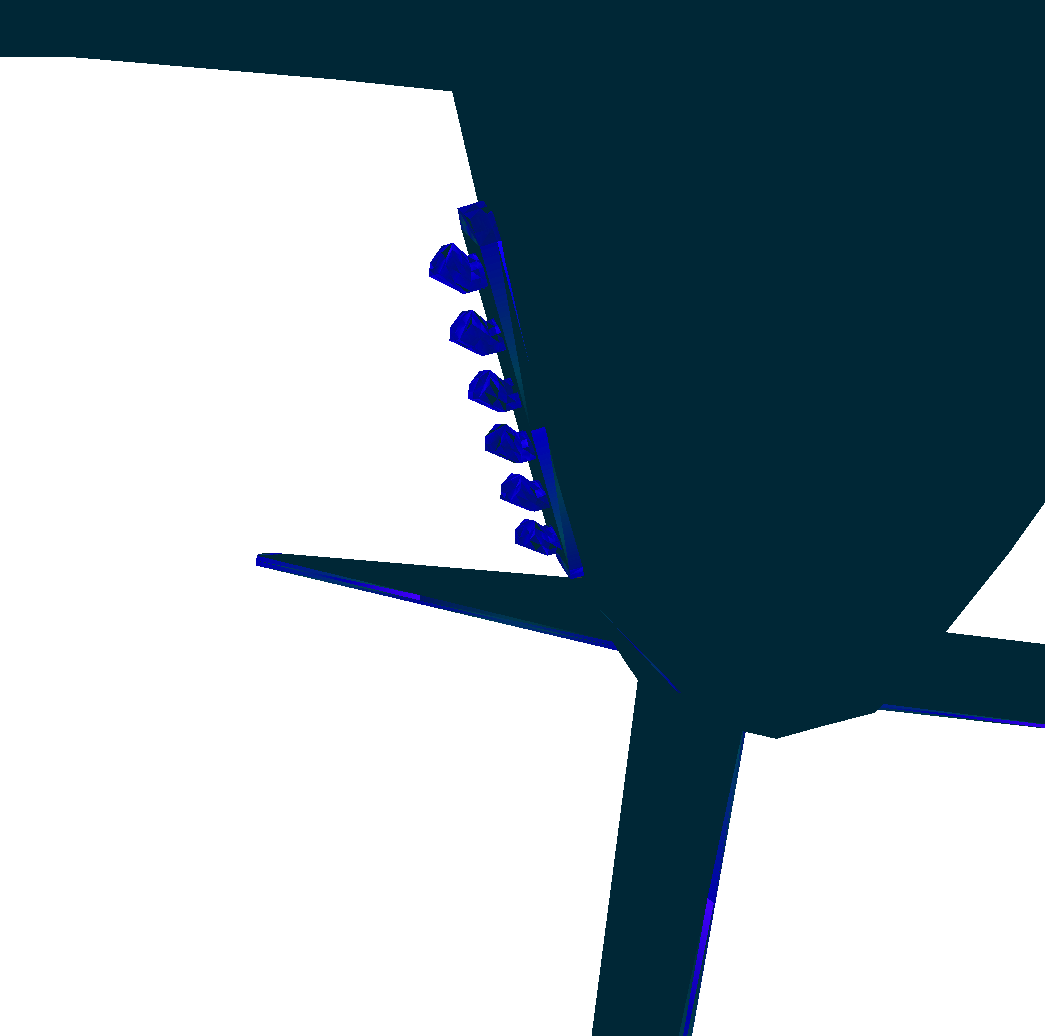
\includegraphics[width=.7\textwidth]{ms_mechanical.png}\\ % PNG-File
	\caption{Perspective detail view on object three (P51)}
	\label{fig:results_ms_mechanical}
\end{figure}

The mapping of colors to \textit{mesh saliency} values in figure \ref{fig:results_ms_mechanical} is similar to that used for all figures shown in section \ref{sec:saliency_and_difference_maps}. The closer the color is to white, the higher \textit{mesh saliency} value is at any given vertex. Again, note that values are not normalised here. The fact that, despite that, most of the object is still shaded nearly black and only small details have seem to be of any importance according to the process, shows that the originally proposed, unaltered version of \textit{mesh saliency} might not be suitable for mechanical objects. Again, this is highly dependent of the object in question and mechanical objects, by nature, can hardly be attributed any common structural pattens.

As mentioned before, the measure of difference suggested in section \ref{sec:measure_of_difference} lacks expressiveness. However, the fact that both raw and weighted overall difference ratios amount to about 0.38 - which is the highest number among the three objects - might indicate that \textit{mesh saliency} has to be greatly altered to produce intuitive results on mechanical objects. Furthermore, even the \textit{user saliency} map for model three was not as distinct as for models one and two. Participants in the user study seemed to have many more, much different interpretations of what parts of an aircraft are \textit{important} than they had regarding animals. So the fact that not much of a statement, other than \textit{saliency maps for mechanical objects will differ stronger than for natural objects} can be made, is not caused by \textit{mesh saliency} possibly not being perfectly suitable for mechanical objects alone.
